\documentclass[11pt,twocolumn]{article}

\usepackage[T1]{fontenc}
\usepackage[english]{babel}
\usepackage[hmarginratio=1:1,top=20mm,bottom=20mm,columnsep=20pt,left=15mm]{geometry}
\usepackage[original]{abstract}
\usepackage{graphicx,hyperref,lipsum}
\usepackage[hang, small,labelfont=bf,up]{caption}
\usepackage{float,wrapfig,subcaption,booktabs,lettrine,enumitem,amsmath}

\renewcommand{\abstractnamefont}{\normalfont\bfseries}
\renewcommand{\abstracttextfont}{\normalfont\small}

\graphicspath{ {./../images/} }

\title{\textbf{Human Language Technlogies \\ Twitter Sentiment Analysis}}
\author{Gianmarco Ricciarelli \\ \href{mailto:gianmarcoricciarelli@gmail.com}{gianmarcoricciarelli@gmail.com}\\
Project's Repository: \href{https://github.com/germz01/twitter_sentiment_analysis}{GitHub}}
\date{}

\begin{document}
    \maketitle

    \begin{abstract}
        \noindent
        Nowadays, when delving into the Social Network landscape, a user can choose among different
        paths, depending on the type of experience he/she is searching. Regardless the type of platform that
        is chosen by the user, either Facebook, or Instagram or Twitter, the amount of textual data that is
        produced every day is massive. With this report, I describe the project I developed for the
        \textit{Human Language Technologies} class hosted by the University of Pisa's Master's Degree in
        Computer Science, that is, a prediction-oriented analysis of two datasets composed by labeled tweets,
        with the second one providing informations also on the tweets' topic, via a series of models like SVM,
        NB, CNN and LSTM.
    \end{abstract}

    \section{Corpora Collection} % (fold)
    \label{sec:corpus_collection}
        The amount of textual data produced by the users on the various Social Networks on a day-by-day
        basis is massive, and, for this reason, it is not too difficult to scrape the web in order to
        build a corpus composed by an acceptable amount of documents. Among all the available platforms, I
        choosed to work with Twitter, since the documents, that is, the tweets, produced by the users are
        limited to be $280$ characters long at most, and since the API that is used for communicating with
        the server is very simple and inuitive to use. In order to properly train the models that I
        wanted to compare, I assembled two corpora of almost $40000$ and $17000$ labeled tweets, respectively, by
        requesting Twitter to download the documents used for the A and B Tasks of the
        \textit{International Workshop on Semantic Evaluation} competitions from $2013$ to $2017$.
        I choosed to work with the documents provided by the SemEval
        competitions because every tweet was hand-labeled by a human, that is, guaranteeing a sound
        catalogation of the sentiments expressed by the tweets. The documents composing the A Task corpus can be
        labeled either as positive, negative or neutral, while the documents composing the B Task corpus can be
        labeled either as positive or negative. Despite the tweets' labels being so well defined, a SemEval
        dataset is quite small if it is taken on its own. This is due to the fact that, since Twitter is a
        very dynamic and constantly upgraded platform, some of the documents provided by each dataset
        were deleted by the users. For this reason I decided to merge the datasets provided by the various
        competitions in order to obtain the final versions of the corpora.
    % section corpus_collection (end)

    \section{Corpus Analysis} % (fold)
    \label{sec:corpus_analysis}
        The original versions of the corpora I assembled was composed by more than $48000$ labeled tweets for the
        A Task corpus, and more than $18000$ for the B Task corpus. As I said before, some of the tweets were
        deleted by the users, resulting in a document containing the 'Not Available' string. Moreover, the
        corpora contained a small percentage of duplicate tweets. By removing the not available tweets and the
        duplicates, I obtained the final version of the corpora composed by $39308$ labeled documents for the
        A Task corpus, and by $16333$ for the B Task corpus. In particular, the obtained corpus for the A Task
        contains:

        \begin{itemize}
            \item $15092$ positive tweets;
            \item $6005$ negative tweets;
            \item $18211$ neutral tweets;
        \end{itemize}

        while the one for the B Task contains:

        \begin{itemize}
            \item $12833$ positive tweets;
            \item $3500$ negative tweets;
        \end{itemize}

        \noindent
        As we can see, the majority of the documents composing the A Task corpus are labeled as neutral, and also
        the positive tweets are very well represented. Conversely, the negative ones are poorly
        represented, and, as we will see, this fact will be crucial for their classification in the
        learning and testing phases of the algorithms I will apply. For the B Task corpus we can see a similar
        situation, in which almost all documents are labeled as positive, while a small percentage are labeled as
        negative. The type of subdivision used for the A Task documents allows the corpus to be considered as
        containing both subjective and objective tweets. By considering this new subdivision, we can see that the
        corpus contains:

        \begin{itemize}
            \item $21097$ subjective tweets;
            \item $18211$ objective tweets;
        \end{itemize}

        \noindent
        This time, both the two sets of documents are well represented. In order to provide a richer
        analysis, I decided to apply the classification algorithms on three types of problems; the
        positive-vs-negative-vs-neutral problem represented by the A Task of the 2017 SemEval competiton, the
        positive-vs-negative problem represented by the B Task of the 2017 SemEval competition and finally the
        subjective-vs-objective problem, which uses the alternative version of the A Task corpus to answer the
        Task considering a different perspective. Before starting with the classification phase, which is
        described in Section \ref{sec:classification}, I studied the A Task corpus in order to have a better
        understanding of the documents composing the dataset. A similar study can be obtained also for the B Task
        corpus, but, since the documents composing the dataset are divided by topic, I think is more interesting
        to analyse the less specific A Task corpus. For starting my analysis, I tokenized the tweets contained in
        the corpus and I observed the distribution of the word frequencies.

        \begin{figure}[h]
            \centering
            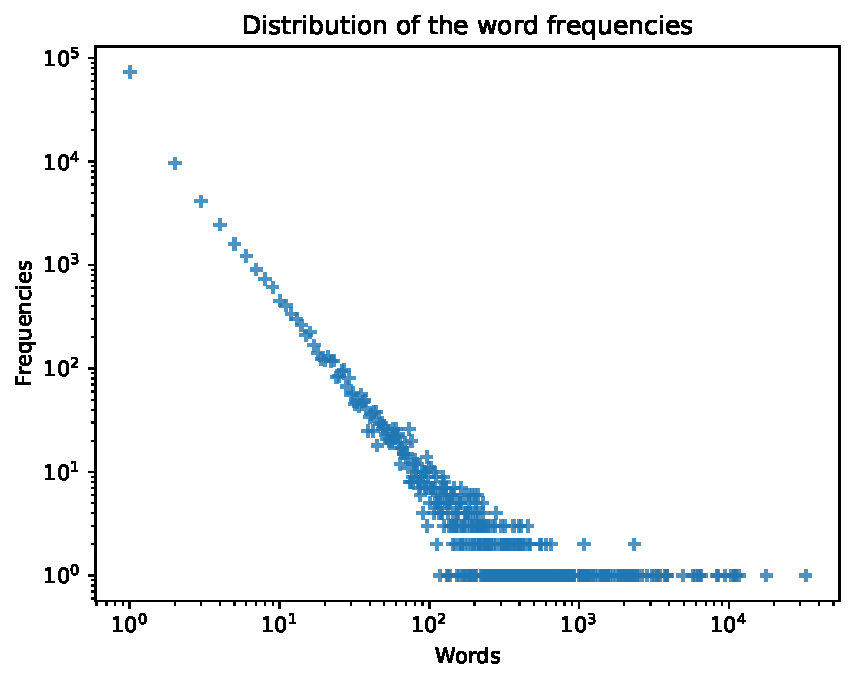
\includegraphics[width=\linewidth]{../images/word_frequencies.pdf}
            \caption{Word Frequencies Distribution.}
            \label{fig:word_frequencies}
        \end{figure}

        \noindent
        As we can see in Figure \ref{fig:word_frequencies}, the words' frequencies follow the well known
        Zipf's law, with a small number of words that appears frenquently, the so called stop words, and the
        majority of the remaining words that appears less and less frenquently. Following the analysis
        proposed in \cite{twitter_as_a_corpus}, I updated the tokens obtained by the early stage of the
        analysis by adding the tags from the application of a Part of Speech Tagging procedure, and I
        observed the tags' distribution between the corpus' documents when considering only the
        positive/negative tweets and the subjective/objective tweets.

        \begin{figure}[h]
            \centering
            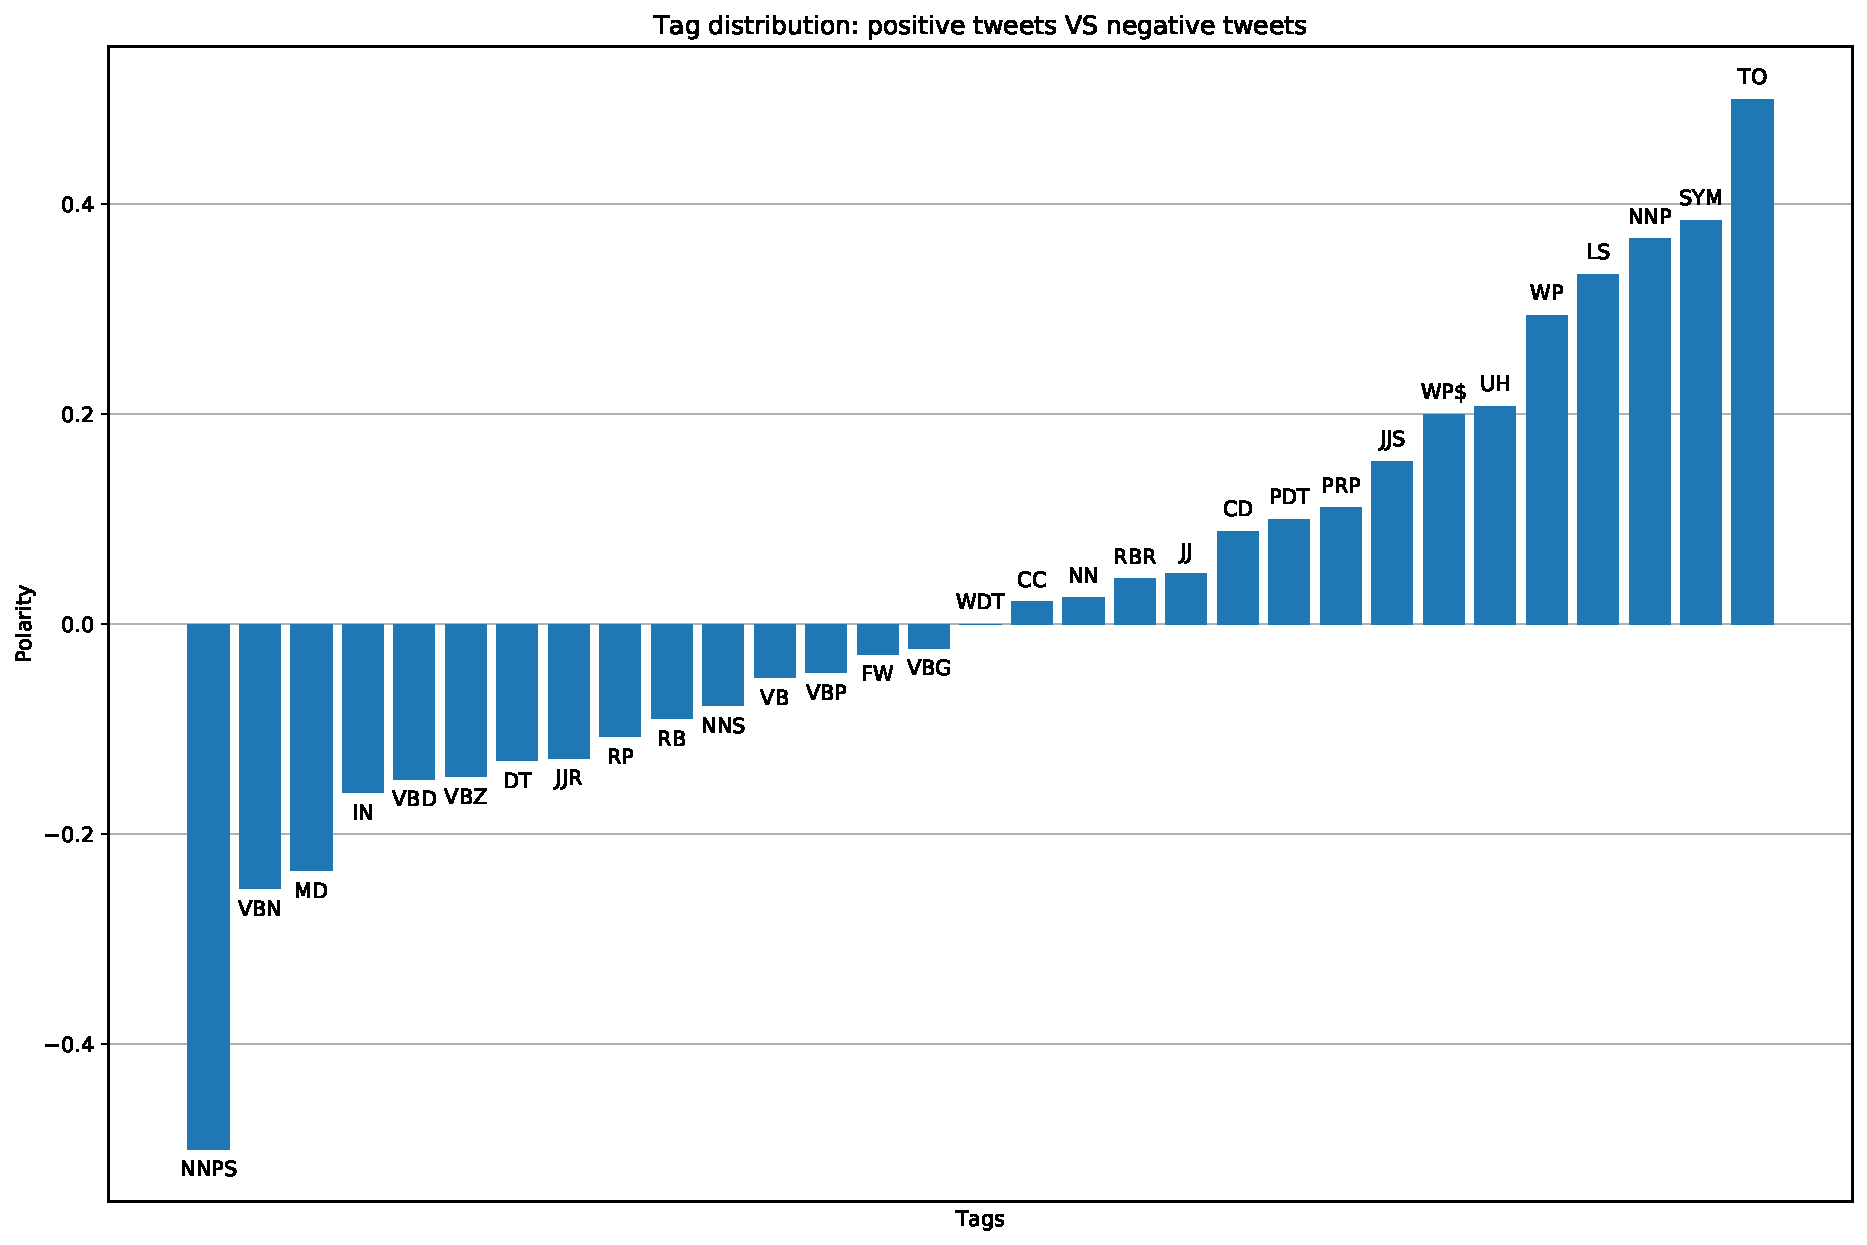
\includegraphics[width=\linewidth]{../images/tag_distribution_positive_vs_negative.pdf}
            \caption{Tag Distribution for Positive and Negative tweets.}
            \label{fig:tags_pos_vs_neg}
        \end{figure}

        \noindent
        As I said before, \cite{twitter_as_a_corpus} proposes the following formula to perform a pairwise
        comparison of tags distributions for each tag and two sets:

        \begin{equation*}
            P_{1, 2}^T = \frac{N_1^T - N_2^T}{N_1^T + N_2^T}
        \end{equation*}

        \noindent
        where $N_1^T$ and $N_2^T$ are numbers of tag $T$ occurrences in the first and second sets respectively.
        As we can see from Figure \ref{fig:tags_pos_vs_neg}, POS tags for positive and negative tweets are not
        distributed evenly, hence we can infer the sentiment behing a document by looking at its tags. We can
        see that the presence of a plural proper noun (NNPS) is a strong indicator for the positive label as
        well as past participle verbs (VBN) and modal (MD). For the negative label, we can see that superlative
        adverbs (RBS) is a strong indicator, as well as List item marker (LS) and possessive wh-pronouns (WP\$).

        \begin{figure}[h]
            \centering
            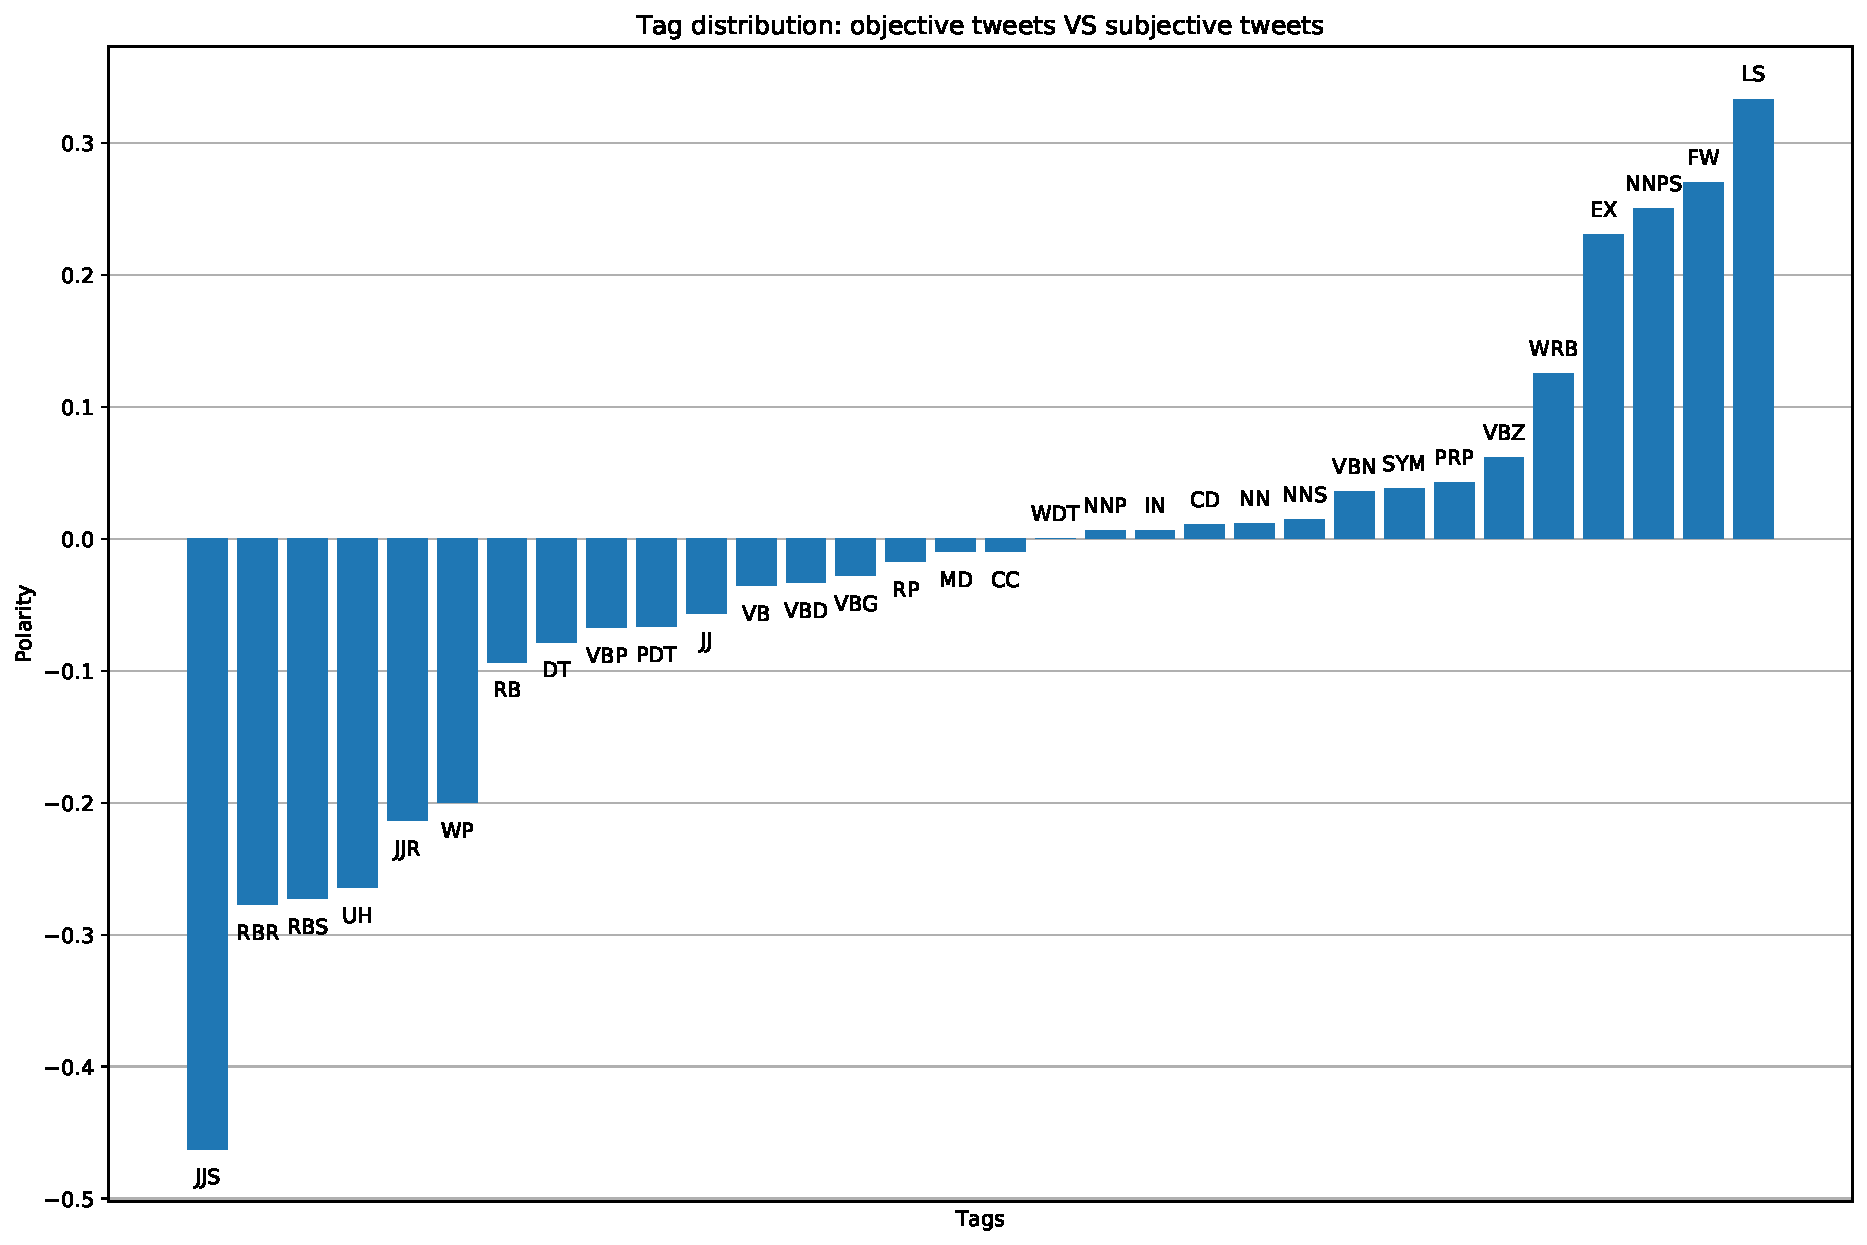
\includegraphics[width=\linewidth]{tag_distribution_objective_vs_subjective.pdf}
            \caption{Tag Distribution for Objective and Subjective tweets.}
            \label{fig:tags_obj_vs_subj}
        \end{figure}

        \noindent
        In Figure \ref{fig:tags_obj_vs_subj} we can observe the tags' distribution for the subjective and
        objective tweets. We can see that possessive superlative adjectives (JJS), comparative adverbs (RBR) and
        superlative adverbs (RBS) are all indicators for objective tweets, while list item markers (LS),
        foreign words (FW) and plural proper nouns (NNPS) are indicators for subjective tweets. Finally, I have
        collected some of the most used words for positive and negative tweets and represented them via
        wordclouds, in order to provide a better understanding of the sentiments that labels the documents
        composing the corpus, and for providing some visual representation of the informations showed with
        Figure \ref{fig:tags_pos_vs_neg} and Figure \ref{fig:tags_obj_vs_subj}.

        \begin{figure}[h]
            \centering
            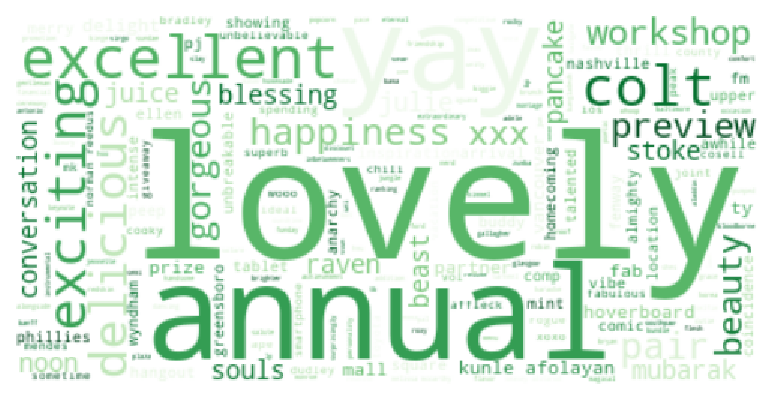
\includegraphics[width=\linewidth]{positive_tokens_wordcloud.pdf}
            \caption{Positive tokens wordcloud.}
            \label{fig:positive_tokens_wordcloud}
        \end{figure}

        \noindent
        In Figure \ref{fig:positive_tokens_wordcloud} we can see the wordcloud for the tokens contained in the
        positive labeled tweets, while in Figure \ref{fig:negative_tokens_wordcloud} we can see the tokens for
        the negative labeled ones.

        \begin{figure}[h]
            \centering
            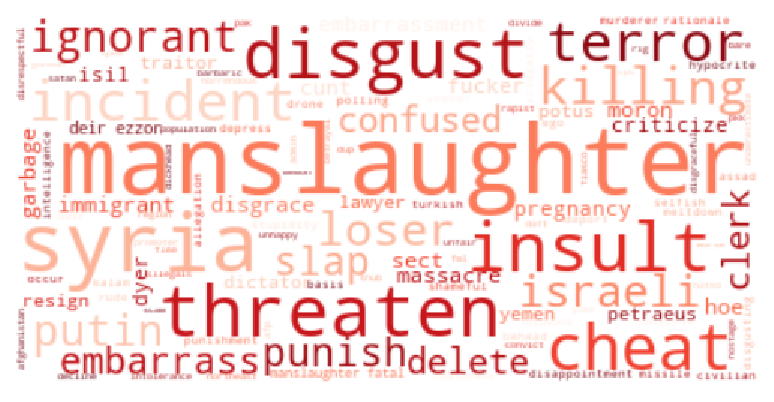
\includegraphics[width=\linewidth]{negative_tokens_wordcloud.pdf}
            \caption{Negative tokens wordcloud}
            \label{fig:negative_tokens_wordcloud}
        \end{figure}
    % section corpus_analysis (end)

    \section{Classification} % (fold)
    \label{sec:classification}
        The Human Language Technologies research's field is very popular at the moment, and, in particular, the
        Sentiment Analysis branch has a rich literature and many tools and resoruces availables for learning.
        Having analysed the obtained corpora, as described in Section \ref{sec:corpus_collection} and Section
        \ref{sec:corpus_analysis}, the next step for my research was to implement a Classification procedure,
        in which I decided to apply some popular Machine Learning models like Support Vector Machines,
        Naïve Bayes, Convolutional Neural Networks and Long Short-term Memory Recurrent Neural Networks, as
        described in \cite{semeval_2014,state_of_the_art,semeval_2016,esuli,attardi}. Being the corpora composed
        of documents labeled with three distinct labels and two distinc labels, respectively, that is, positive,
        negative and neutral, and positive and negative, I decided to direct the Classification phase towards the
        takling of three different tasks:

        \begin{itemize}
            \item Classification of positive tweets vs negative tweets as in the B Task of 2017 SemEval
            competition;
            \item Classification of positive tweets vs negative tweets vs neutral tweets as in the A Task of the
            2017 SemEval competition;
            \item Classification of subjective tweets vs objective tweets, similar to the A Task of the 2017
            SemEval competition, but with a dataset composed by documents that are either subjective
            (positive or negative) or objective (neutral);
        \end{itemize}

        \noindent
        As in a typical Machine Learning procedure, the documents composing the corpus cannot be fed directly to
        the models, since they are texts, and not numbers, so, before applying the algorithms, I developed a
        preprocessing routine, in which I developed the conversion from texts understandable by humans to texts
        understandable by machines. After preprocessing the corpus I validated each one of the learners via the
        application of well-known validation techniques like K-Fold Cross Validation and Random Grid Search.
        Finally, for each one of the three tasks, I collected and compared the results provided by the
        application of the various learning algorithms.

        \subsection{Preprocessing Routine} % (fold)
        \label{sub:preprocessing_routine}
            As I said before, there are plenty of resources for learning about Human Language Technologies, and,
            in general, Sentiment Analysis. After reading about the subject, I developed a Preprocessing
            Routine that is composed by the following steps:

            \begin{enumerate}
                \item Tokenization: the original documents are splitted into tokens via the
                \href{https://www.nltk.org/api/nltk.tokenize.html#module-nltk.tokenize}{TweetTokenizer}
                tokenizer provided by \href{https://www.nltk.org/py-modindex.html}{NLTK}. This tokenizer is
                specifically trained to work on tweets;
                \item Part Of Speech Tagging: each token list is tagged via the application of a POS
                tagger, also provided by NLTK;
                \item Cleaning: for each token list, the token that are not alphanumeric and that contains
                stop words are removed;
                \item Lemmatization: each one of the token that came out of the Cleaning phase is transformed
                in its original lemma;
            \end{enumerate}

            \noindent
            As an example, if we apply the Preprocessing Routine to the document:\\

            \noindent
            \texttt{April has to live. Sharknado wouldn't be the same without her tiny chainsaw. \#aprillives},
            \\

            \noindent
            we obtain the token list: \\

            \noindent
            \texttt{['april', 'live', 'sharknado', 'without', 'tiny', 'chainsaw']}.
        % subsection preprocessing_routine (end)

        \subsection{Pipeline} % (fold)
        \label{sub:pipeline}
            Before feeding the corpora to the Naïve Bayes and Support Vector Machine classifiers I further
            preprocessed the documents via the application of a Pipeline composed by:

            \begin{enumerate}
                \item A Vectorizer, that is, the
                \href{https://scikit-learn.org/stable/modules/generated/sklearn.feature_extraction.text.CountVectorizer.html#sklearn.feature_extraction.text.CountVectorizer}{CountVectorizer}
                provided by
                \href{https://scikit-learn.org/stable/index.html}{scikit-learn}, which takes in input
                the tokenized documents from the Preprocessing Routine and, for each tweet, returns a list
                of integers where each integer corresponds to a word in the tweet;
                \item A Transformer, that is, the
                \href{https://scikit-learn.org/stable/modules/generated/sklearn.feature_extraction.text.TfidfVectorizer.html#sklearn.feature_extraction.text.TfidfVectorizer}{TfidfTransformer}
                provided by scikit-learn, which takes the matrix created by the Vectorizer and
                transform it to a normalized or tf-idf representation;
                \item A Selectioner, that is, the
                \href{https://scikit-learn.org/stable/modules/generated/sklearn.feature_selection.SelectKBest.html}{SelectKBest} provided by scikit-learn, which
                takes the output of the Transformer and select the k most representative features via the
                application of the chi-squared test;
            \end{enumerate}

            \noindent
            Moreover, for the Selectioner, the number of features selected, that is, the k parameter,
            ranges between $1000$ and $5000$. This parameter is adapted depending on the task during the
            Validation Routine, which is described in the next section.
        % subsection pipeline (end)

        \subsection{Validation Routine} % (fold)
        \label{sub:validation_routine}
            Every Machine Learning algorithm is characterized by a number of parameters, that is, the
            so-called hyperparameters, that the user can modify accordingly to the type of task he/she is
            takling. Being the task of tuning every single hyperparameter a cumbersome one, I decided to
            apply the well-know Random Grid Search technique, as described in \cite{random_grid_search}, in
            order to discover the most effective combination of hyperparameters for the models I want to
            compare. I used the $70\%$ of the corpora as a training set, while the remaining $30\%$ was used as
            validation set. Before validating, for each "point" produced by the Random Grid Search, I
            applied the K-Fold Cross Validation technique, setting the value for the K parameter to $3$.
            Moreover, since the performance of algorithms like the Convolutional Neural Networks and the
            Long Short-term Memory Recurrent Neural Networks are greately influenced by the network's
            architecture, I decided, in order to ease the validation process for each one of the two
            algorithms, to fix a simple architecture and to apply the validation techniques to that fixed
            structure for obtaining the best results. The architecture I selected for the CNN is composed
            by an Embedding Layer, followed by a Convolutional Layer, a Max Pooling and finally by a Fully
            Connected Neural Network. The architecture I selected for the LSTM is composed by an Embedding
            Layer, followed by a LSTM Layer and finally by a Fully Connected Neural Network For enriching
            my analysis of the models' performances, I used and validated three types of word embeddings
            for the CNN and the LSTM algorithms:

            \begin{itemize}
                \item a word embedding learned during the training phase with $300$ entries for each word;
                \item the GloVe \cite{glove} pre-trained word vectors with $300$ entries for each word;
                \item the fastText \cite{fasttext} pre-trained word vectors with $300$ entries for each
                word;
            \end{itemize}

            \noindent
            For now on, I will refer to the CNN/LSTM using the word embeddings learned during the training
            phase with the subscript A, while I will use the subscript G for the GloVe pre-trained word
            vectors and F for the fastText pre-trained word vectors, respectively.
        % subsection validation_routine (end)

        \subsection{Positive vs Negative Classification} % (fold)
        \label{sub:positive_vs_negative_classification}
            As we might think, this is the easier one among the tasks I have decided to approach. This is
            because it is essentially a binary classification problem applied to a set of very small datasets,
            each one representing a topic, hence resulting in a easier classification from the Machine Learning
            point of view.

                \begin{table}[h]
                     \centering
                     \begin{tabular}{| c | c |}
                        \hline
                        \textbf{Classifier} & \textbf{Score} \\
                        \hline
                        $SVM$ & $0.64$ \\
                        \hline
                        $NB$ & $0.65$ \\
                        \hline
                        $CNN_A$ & $0.68$ \\
                        \hline
                        $CNN_G$ & $0.65$ \\
                        \hline
                        $CNN_F$ & $0.67$ \\
                        \hline
                        $LSTM_A$ & $0.77$ \\
                        \hline
                        $LSTM_G$ & $0.64$ \\
                        \hline
                        $LSTM_F$ & $0.62$ \\
                        \hline
                    \end{tabular}
                    \caption{Models' comparison for the positive-vs-negative classification task.}
                    \label{tab:pn_comparison}
                \end{table}

            \noindent
            In Table \ref{tab:pn_comparison} we can see the results for the application
            of the models to the B Task corpus containing only positive and negative documents. The score for
            each one of the classifiers is obtained by via the following formula:

            \begin{equation*}
                \rho^{PN} =\frac{1}{2}(\rho^{P} + \rho^{N}) = \frac{1}{2}
                \left ( \frac{PP}{PP + NP} + \frac{NN}{NN + PN} \right )
            \end{equation*}

            \noindent
            where $\rho^{P}$ and $\rho^{N}$ are the positive and negative class recall, respectively. Each
            classifier computes this score for every topic, and the mean value is reported as the final score.
            As we can  see, in general, the score is above $0.60$. The higher score is
            reached by the LSTM using a word embedding learned during the training phase and by the CNN using a
            word embedding learned during the training phase, while the worst score is obtained by the LSTM using
            the fastText pre-trained word vectors.
        % subsection positive_vs_negative_classification (end)

        \subsection{Positive vs Negative vs Neutral Classification} % (fold)
        \label{sub:positive_vs_negative_vs_neutral_classification}
            In order to takle this task, the entire corpus is preprocessed as described in Section
            \ref{sub:preprocessing_routine}. This type of task results to be more difficult compared to
            the one described in Section \ref{sub:positive_vs_negative_classification}, both in term of
            time and computational resources.

            \begin{table}[h]
                \centering
                \begin{tabular}{| c | c |}
                    \hline
                    \textbf{Classifier} & \textbf{Score} \\
                    \hline
                    $SVM$ & $0.51$ \\
                    \hline
                    $NB$ & $0.51$ \\
                    \hline
                    $CNN_A$ & $0.65$ \\
                    \hline
                    $CNN_G$ & $0.60$ \\
                    \hline
                    $CNN_F$ & $0.61$ \\
                    \hline
                    $LSTM_A$ & $0.71$ \\
                    \hline
                    $LSTM_G$ & $0.61$ \\
                    \hline
                    $LSTM_F$ & $0.54$ \\
                    \hline
                \end{tabular}
                \caption{Models' comparison for the positive-vs-negative-vs-neutral classification task.}
                \label{tab:a_comparison}
            \end{table}

            \noindent
            In Table \ref{tab:a_comparison} we can see the results of the application of the models to the A Task
            corpus. The score for each one of the classifiers is obtained by via the following formula:

            \begin{equation*}
                F_1^{PN} = \frac{F_1^P + F_1^N}{2}
            \end{equation*}

            \noindent
            where $F_1^P$ and $F_1^N$ are the $F_1$ score for the positive and negative class, respectively.
            As we can see, in general, the score tend to be greater
            than $0.50$. This time the best models are, respectively, the LSTM using a word embedding learned
            during the training phase and the CNN using word embeddings learned during the training phase, while
            the worst models are the SVM model and the NB model.
        % subsection positive_vs_negative_vs_neutral_classification (end)

        \subsection{Subjective vs Objective Classification} % (fold)
        \label{sub:subjective_vs_objective_classification}
            Finally I discuss the last of the tasks that I takled for my project, that is, the
            classification of subjective and objective tweets using the A Task corpus. For the tasks described in
            Sections \ref{sub:positive_vs_negative_classification} and
            \ref{sub:positive_vs_negative_vs_neutral_classification} the labels were substituted with
            positive integers from $0$ to $1$ for the positive-vs-negative classification, and from $0$ to
            $2$ for the positive-vs-negative-vs-neutral classification. For this type of classification I
            labeled all the positive and negative documents, that is, the subjective ones, with the integer
            $0$, while the neutral ones, that is, the objective ones, were labeled with the integer $1$.
            As for the task described in Section \ref{sub:positive_vs_negative_vs_neutral_classification},
            also for this task the request in terms of time and computational resources was high.

            \begin{table}[h]
                \centering
                \begin{tabular}{| c | c |}
                    \hline
                    \textbf{Classifier} & \textbf{Score} \\
                    \hline
                    $SVM$ & $0.67$ \\
                    \hline
                    $NB$ & $0.65$ \\
                    \hline
                    $CNN_A$ & $0.78$ \\
                    \hline
                    $CNN_G$ & $0.70$ \\
                    \hline
                    $CNN_F$ & $0.68$ \\
                    \hline
                    $LSTM_A$ & $0.77$ \\
                    \hline
                    $LSTM_G$ & $0.68$ \\
                    \hline
                    $LSTM_F$ & $0.69$ \\
                    \hline
                \end{tabular}
                \caption{Models' comparison for the subjective-vs-objective classification task.}
                \label{tab:so_comparison}
            \end{table}

            \noindent
            In Table \ref{tab:so_comparison} we can see the results for the application
            of the models to the A Task corpus composed by subjective and objective tweets. For obtaining the
            score, each classifier applied the formula described in Section
            \ref{sub:positive_vs_negative_classification}, being this a binary classification task, and not a
            multilabel classification task as the one described in Section
            \ref{sub:positive_vs_negative_vs_neutral_classification} We can see that the best model is
            represented by a CNN using word embeddings learned during the training phase, followed closely by a
            LSTM using word embeddings learned during the training phase. The worst score is obtained by the NB
            model.
        % subsection subjective_vs_objective_classification (end)
    % section classification (end)

    \section{Conclusions} % (fold)
    \label{sec:conclusions}
        The Sentiment Analysis research field is very active at the moment, with a great number of paper
        available and many tools and resources that can be used for learning and enriching our knowledge
        about the subject. The possibility to freely access great and constantly updated amount of data, like, for
        example, Twitter's tweets, Facebook's posts, screenplays, etc. etc., makes it easy to experiment
        with the available models or even to create new ones in order to obtain better performances in
        comparison with the old ones. With this project I learned about how to obtain a good amount of
        documents from a reliable source, which in this case is represented by the
        \textit{International Workshop on Semantic Evaluation}, how to analyze textual data in order to
        discover hidden relationships between the documents composing a corpus, and, most importantly, I
        learned how to use well-know models like Support Vector Machines, Naïve Bayes, Convolutional Neural
        Networks and Long Short-term Memory Recurrent Neural Networks in order to classify the sentiment
        behind a document written by an human user, which nowadays can be an useful resource to be used
        in a variety of application's fields. I think that the performances I obtained for the CNNs and LSTMs
        might be upgraded via the use of different architectures, but, as I said before, for my project I
        preferred a simpler approach.
    % section conclusions (end)

    \begin{thebibliography}{9}
        \bibitem{twitter_as_a_corpus}
        Pak, Alexander \& Paroubek, Patrick. (2010). Twitter as a Corpus for Sentiment Analysis and Opinion
        Mining. Proceedings of LREC. 10.

        \bibitem{semeval_2014}
        Nakov, P. \& Rosenthal, S. \& Kiritchenko, S. et al. Developing a successful SemEval task in sentiment
        analysis of Twitter and other social media texts. Lang Resources \& Evaluation 50, 35–65 (2016).
        https://doi.org/10.1007/s10579-015-9328-1

        \bibitem{state_of_the_art}
        Mohammad, Saif \& Kiritchenko, Svetlana \& Zhu, Xiaodan. NRC-Canada: Building the State-of-the-Art in
        Sentiment Analysis of Tweets. Second Joint Conference on Lexical and Computational Semantics,
        Volume 2: Proceedings of the Seventh International Workshop on Semantic Evaluation,
        June 2013, Atlanta, Georgia, USA.

        \bibitem{semeval_2016}
        Nakov, Preslav \& Ritter, Alan \& Rosenthal, Sara \& Sebastiani, Fabrizio \& Stoyanov, Veselin.
        SemEval-2016 Task 4: Sentiment Analysis in Twitter. Proceedings of the 10th International Workshop on
        Semantic Evaluation (SemEval-2016), June 2016, San Diego, California.

        \bibitem{esuli}
        Esuli, Andrea. ISTI-CNR at SemEval-2016 Task 4: Quantification on an Ordinal Scale. Proceedings of the
        10th International Workshop on Semantic Evaluation (SemEval-2016), June 2016. Association for
        Computational Linguistics, San Diego, California.

        \bibitem{attardi}
        Attardi, Giuseppe \& Sartiano, Daniele. (2016). UniPI at SemEval-2016 Task 4: Convolutional Neural
        Networks for Sentiment Classification. 220-224. 10.18653/v1/S16-1033.

        \bibitem{random_grid_search}
        James Bergstra and Yoshua Bengio. 2012. Random search for hyper-parameter optimization. J. Mach. Learn.
        Res. 13, 1 (February 2012), 281–305.

        \bibitem{glove}
        Jeffrey Pennington \& Richard Socher \& Christopher D. Manning. GloVe: Global Vectors for Word
        Representation. Empirical Methods in Natural Language Processing (EMNLP), 2014, 1532--1543
        http://www.aclweb.org/anthology/D14-1162

        \bibitem{fasttext}
        Mikolov, Tomas \& Grave, Edouard \& Bojanowski, Piotr \& Puhrsch, Christian \& Joulin, Armand.
        Advances in Pre-Training Distributed Word Representations. Proceedings of the International Conference
        on Language Resources and Evaluation (LREC 2018), 2018.
    \end{thebibliography}
\end{document}
